\section{Testing and Validation}
This section details the tests that were conducting on the TSC module while it is connected to the ADC and HUB module.
The tests conducted were only aimed to prove the functionality of the module and weren't aimed to test the module protection of misuse, even-though the TSC module was written to handle such cases.

The test bench runs a simple test of sending a pulse on the reset line followed by a pulse on the start line to move the module into running mode.
The module will next get triggered by one of the 256 ADC values going above the TRIGVL.
The TRIGVL is set at 0xC8 and there are only two values in the ADC csv file which are above 0xC0 which are the 150th and 200th values.
The test bench is programmed to send a start pulse on the first trigger and an SBF pulse on any subsequent triggers.

The test was run as one continuous test and several snippets of gktwave were taken and explained in chronological order.

\subsection{Reseting and Starting}
\begin{figure}[H]
    \centering
    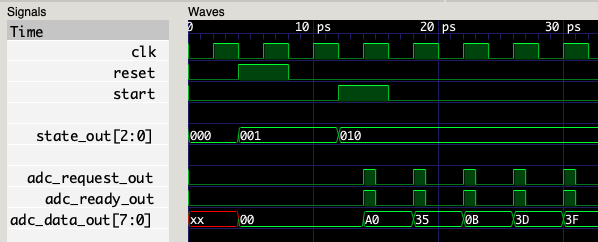
\includegraphics[width=\columnwidth]{Figures/Areset_start_adc}
    \caption{Resetting and Starting gktwave Output}
    \label{fig:testA}
\end{figure}

Firstly, a reset then start pulse are sent and the TSC module response by changing the state from STOP (0b000) to READY (0b001) and then to RUNNING (0b010).
Once the module has entered running mode, it correctly requests data from the the ADC module every rising clock edge, and the adc replies by pulling the ready line high and outputs a new byte on the data bus.
In a real world implementation of this there would be a slight delay between the request being pulled high and the ready begin pulled high.
Next, the TSC module acknowledges the adc ready and resets the request line.
Again, in a real world implementation there would be a slight delay between these edges.

\subsection{Ring Buffer Writing}\label{subsec:ring-buffer-writing}
\begin{figure}[H]
    \centering
    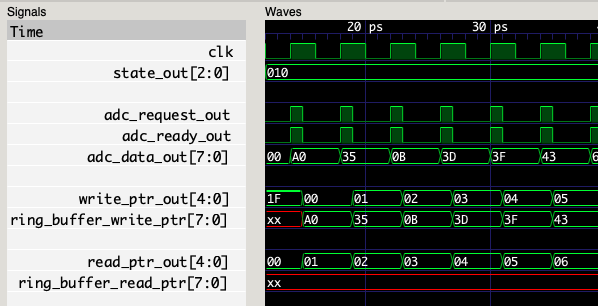
\includegraphics[width=\columnwidth]{Figures/Badc_ring_buffer_write}
    \caption{Ring Buffer Writing gktwave Output}
    \label{fig:testB}
\end{figure}

In RUNNING state, the adc value is written into the ring buffer.
As it is shown in \fref{fig:testB}, the first byte the ADC module is 0xA0 which is correctly written into address 0 of the ring buffer, and the second byte 0x35 is written into address 1 of the ring buffer, etc.
The byte at the read buffer pointer is unknown at it has not been written yet, and will only output a known value once a full loop of the ring buffer has been written.

\subsection{Ring Buffer Reading}
\begin{figure}[H]
    \centering
    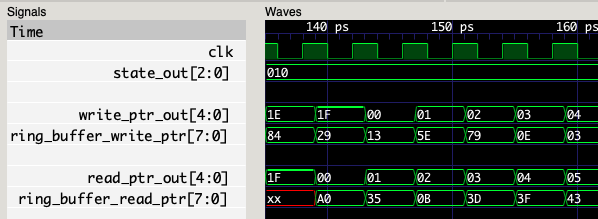
\includegraphics[width=\columnwidth]{Figures/Cadc_ring_buffer_read}
    \caption{Ring Buffer Reading gktwave Output}
    \label{fig:testC}
\end{figure}

As mentioned in \ssref{subsec:ring-buffer-writing}, a full loop has been written into the ring buffer and the read pointer is correctly return 0xA0 for address 0, and 0x35 for address 1, etc.

\subsection{Triggering}
\begin{figure}[H]
    \centering
    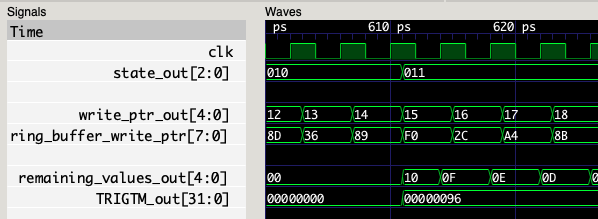
\includegraphics[width=\columnwidth]{Figures/Dtriggered}
    \caption{Triggering gktwave Output}
    \label{fig:testD}
\end{figure}
\begin{figure}[H]
    \centering
    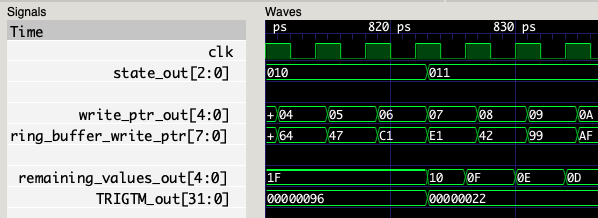
\includegraphics[width=\columnwidth]{Figures/Dtriggered2}
    \caption{Re-triggering gktwave Output}
    \label{fig:testD2}
\end{figure}

\fref{fig:testD} and \fref{fig:testD2} show an initial triggering and re-triggering of the TSC module respectively.
At the point of triggering, the state correctly changes to TRIGGERED (0b011) and the remaining ADC values is set to 16 to indicate that there are 16 more adc values to be written into the ring buffer.
The remaining values then starts counting down with every adc value saved to the ring buffer.
Additionally, the TRGRTM for the initial trigger is correctly updated to the current value of the timer which is:

$\frac{trigger\ time - start\ time}{clock\ period} = \frac{612ps - 12ps }{4ps} = 150 = \mathrm{0x96}$

\subsection{Raising TRD Line}
\begin{figure}[H]
    \centering
    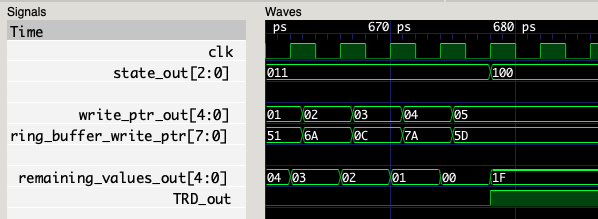
\includegraphics[width=\columnwidth]{Figures/E16captured}
    \caption{Raising TRD Line gktwave Output}
    \label{fig:testE}
\end{figure}

Once there are no remaining values (the remaining value register has reached 0), the TSC module correctly changes state to IDLE (0b100), stops recording adc values, and pulls the TRD line to the HUB module high.

\subsection{Starting or Transmitting From Idle}
\begin{figure}[H]
    \centering
    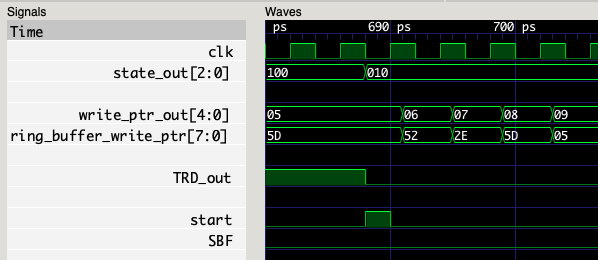
\includegraphics[width=\columnwidth]{Figures/Fidle_start}
    \caption{Starting From Idle gktwave Output}
    \label{fig:testF}
\end{figure}
\begin{figure}[H]
    \centering
    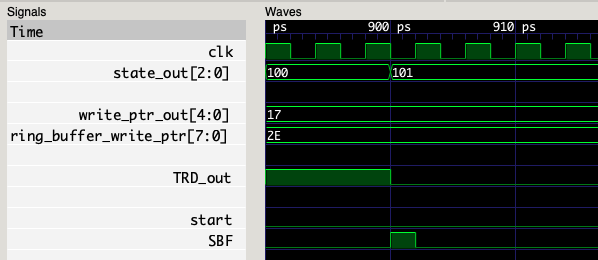
\includegraphics[width=\columnwidth]{Figures/Gidle_SBF}
    \caption{Transmitting Data From Idle gktwave Output}
    \label{fig:testG}
\end{figure}

From the IDLE state, the TSC module can either transition back to RUNNING state or into SENDING state depending on the next command sent.
In \fref{fig:testF}, the TSC module receives a start pulse, correctly transitions back to RUNNING (0b010) state, and correctly continues writing the ADC values into the ring buffer.
In \fref{fig:testG}, the TSC module receives a SBF pulse, correctly transition into SENDING (0b101) state, and starts transmitting data with is shown in \ssref{subsec:starting-data-transmission}.

\subsection{Starting Data Transmission}\label{subsec:starting-data-transmission}
\begin{figure}[H]
    \centering
    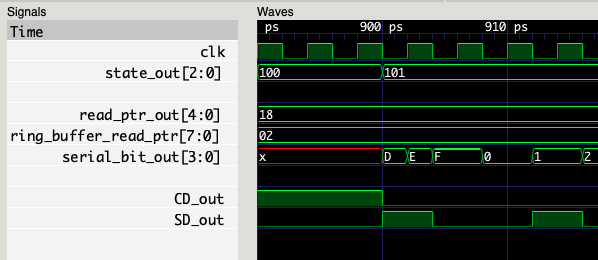
\includegraphics[width=\columnwidth]{Figures/Htransmit_start}
    \caption{Starting Data Transmission gktwave Output}
    \label{fig:testH}
\end{figure}

As the module transitions into SENDING (0b101) state, it immediately pulls CD low and SD high as required; it also sets the serial bit to WAIT (0xD).
When the serial bit is WAIT, it is waiting for the next rising clock edge before it transitions into the TRANSMISSION\_START\_BIT (0xE) which occurs at 902 ps.
Once CD has been low and SD has been high for at least one rising clock edge, the first byte can be sent, which is explained in \ssref{subsec:byte-transmitting}.

\subsection{Byte Transmitting}\label{subsec:byte-transmitting}
\begin{figure}[H]
    \centering
    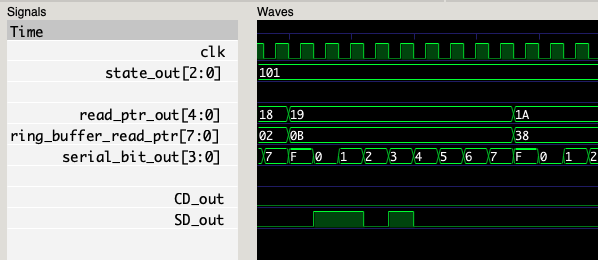
\includegraphics[width=\columnwidth]{Figures/Ibyte_transmit}
    \caption{Byte Transmitting gktwave Output}
    \label{fig:testI}
\end{figure}

The HUB module reads data on the rising clock edge, therefore the TSC module must write data on the falling clock edge, which is shown in \fref{fig:testI} by the SD line only changing with the falling edge clock.
Additionally, each byte is preceded by a low START\_BIT (0xF).

Little Endian encoding was chosen for sending the data on the SD line, so reading the data on the rising edge of the clock as the HUB module would give 0-1101-0000.
This is equivalent to the value 0b0000-1011 = 0x0B which shows that the TSC module correctly sent the byte in the 19th address of the ring buffer.

\subsection{Ending Data Transmission}
\begin{figure}[H]
    \centering
    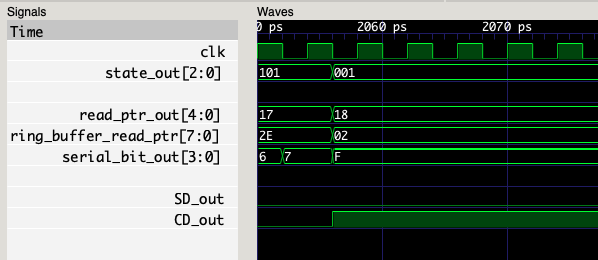
\includegraphics[width=\columnwidth]{Figures/Jtransmit_end}
    \caption{Ending Data Transmission gktwave Output}
    \label{fig:testJ}
\end{figure}

\fref{fig:testH} shows that the first byte transmitted was at address 18, and \fref{fig:testJ} shows that the byte at address 17 has just been transmitted which means the full 32 byte ring buffer has been transmitted.
The TSC module correctly recognises this by dropping the SD line low, pulling the CD line high, resetting the read pointer back to just in front of the write pointer, and finally setting the state back to READY (0b001), waiting to receive a start command once again.